\documentclass[a4paper,10pt]{report}
\usepackage{Cours}
\usepackage{delarray}
\usepackage{fancybox}
\newcommand{\Sum}[2]{\ensuremath{\textstyle{\sum\limits_{#1}^{#2}}}}
\newcommand{\Int}[2]{\ensuremath{\mathchoice%
	{{\displaystyle\int_{#1}^{#2}}}
	{{\displaystyle\int_{#1}^{#2}}}
	{\int_{#1}^{#2}}
	{\int_{#1}^{#2}}
	}}
\usepackage{pstricks-add}



\begin{document}
% \everymath{\displaystyle}

\maketitle{Chapitre 17}{Équations différentielles}

\noindent Dans tout le chapitre, $I$ est un intervalle de $\mathbb{R}$ contenant au moins deux éléments. La notation $\mathbb{K}$ désignera $\mathbb{R}$ ou $\mathbb{C}$ et $n,p$ sont deux entiers naturels non nul.

\section{Équations différentielles scalaires linéaires d'ordre $1$}
\subsection{Définition} 

\begin{defin} Soient $\alpha$, $\beta$ et $\gamma$ trois fonctions définies sur $I$ à valeurs dans $\mathbb{K}$. L'équation 
$$ (\mathcal{E}) \, : \, \alpha y'+\beta y= \gamma$$
est appelée \textit{équation différentielle linéaire d'ordre} $1$, d'inconnue $y$.

\noindent Une \textit{solution} de $(\mathcal{E})$ est une fonction $y : I \rightarrow \mathbb{K}$ dérivable telle que pour tout $t \in I$,
$$ \alpha(t)y'(t)+\beta(t)y(t) = \gamma(t)$$
\end{defin}

\begin{rems}
\item On utilise souvent des abus de notation en confondant $\alpha$ et $\alpha(t)$, $\beta$ et $\beta(t)$... Par exemple, on peux considérer l'équation différentielle suivante :
$$ (1+t^2)y'+ty=t$$
\item On peut aussi définir une solution comme un couple $(y,J)$ où $y$ est solution de l'équation différentielle uniquement sur un sous-intervalle $J \subset I$.
\item On associe parfois les solutions à leurs graphes : on les appelle les \textit{courbes intégrales} associées à l'équation $(\mathcal{E})$.
\end{rems}

\medskip

\begin{defin} Reprenons les notations de la définition précédente.

\begin{itemize}
\item L'équation $(\mathcal{E})$ est dite \textit{homogène} si $\gamma$ est la fonction nulle sur $I$.
\item L'équation $(\mathcal{E})$ est dite à \textit{coefficients constants} si $\alpha$ et $\beta$ sont des fonctions constantes.
\end{itemize}
\end{defin}

\noindent Si la fonction $\alpha$ ne s'annule pas sur $I$, l'équation $(\mathcal{E})$ est alors équivalente à l'équation :
$$ y+ay'=b$$
où $a = \dfrac{\beta}{\alpha}$ et $b = \dfrac{\gamma}{\alpha} \cdot$

\medskip

\noindent On se ramène à ce cas pour le moment.

\begin{defin} On appelle \textit{problème de Cauchy} tout système de la forme :
$$ \left\lbrace \begin{array}{ccl}
y'+ay=b \\
y(t_0)=y_0 \\
\end{array}\right.$$
où :
\begin{itemize}
\item $a$ et $b$ sont des fonctions définies sur $I$ à valeurs dans $\mathbb{K}$.
\item $t_0$ est un élément de $I$ et $y_0 \in \mathbb{K}$.
\end{itemize}
\end{defin}

\begin{thm}[Cauchy-Lipschitz linéaire] Si $a$ et $b$ sont des fonctions continues sur $I$ alors le problème de Cauchy précédent admet une unique solution.
\end{thm}

\begin{rem} L'unicité d'une solution vérifiant la condition $y(t_0)=y_0$ signifie que si deux solutions coincident en un point alors elles coïncident partout. Autrement dit, les courbes intégrales ne se coupent pas.
\end{rem}

\pagebreak

\begin{center}
\textbf{Courbes intégrales associées à $y'+ay+1=0$ }
\end{center}

\begin{multicols}{2}
\begin{center}
$a=1$ et $y(0) \in \lbrace -3,-2,-1,0,1,2 \rbrace$
\end{center}
\begin{center}
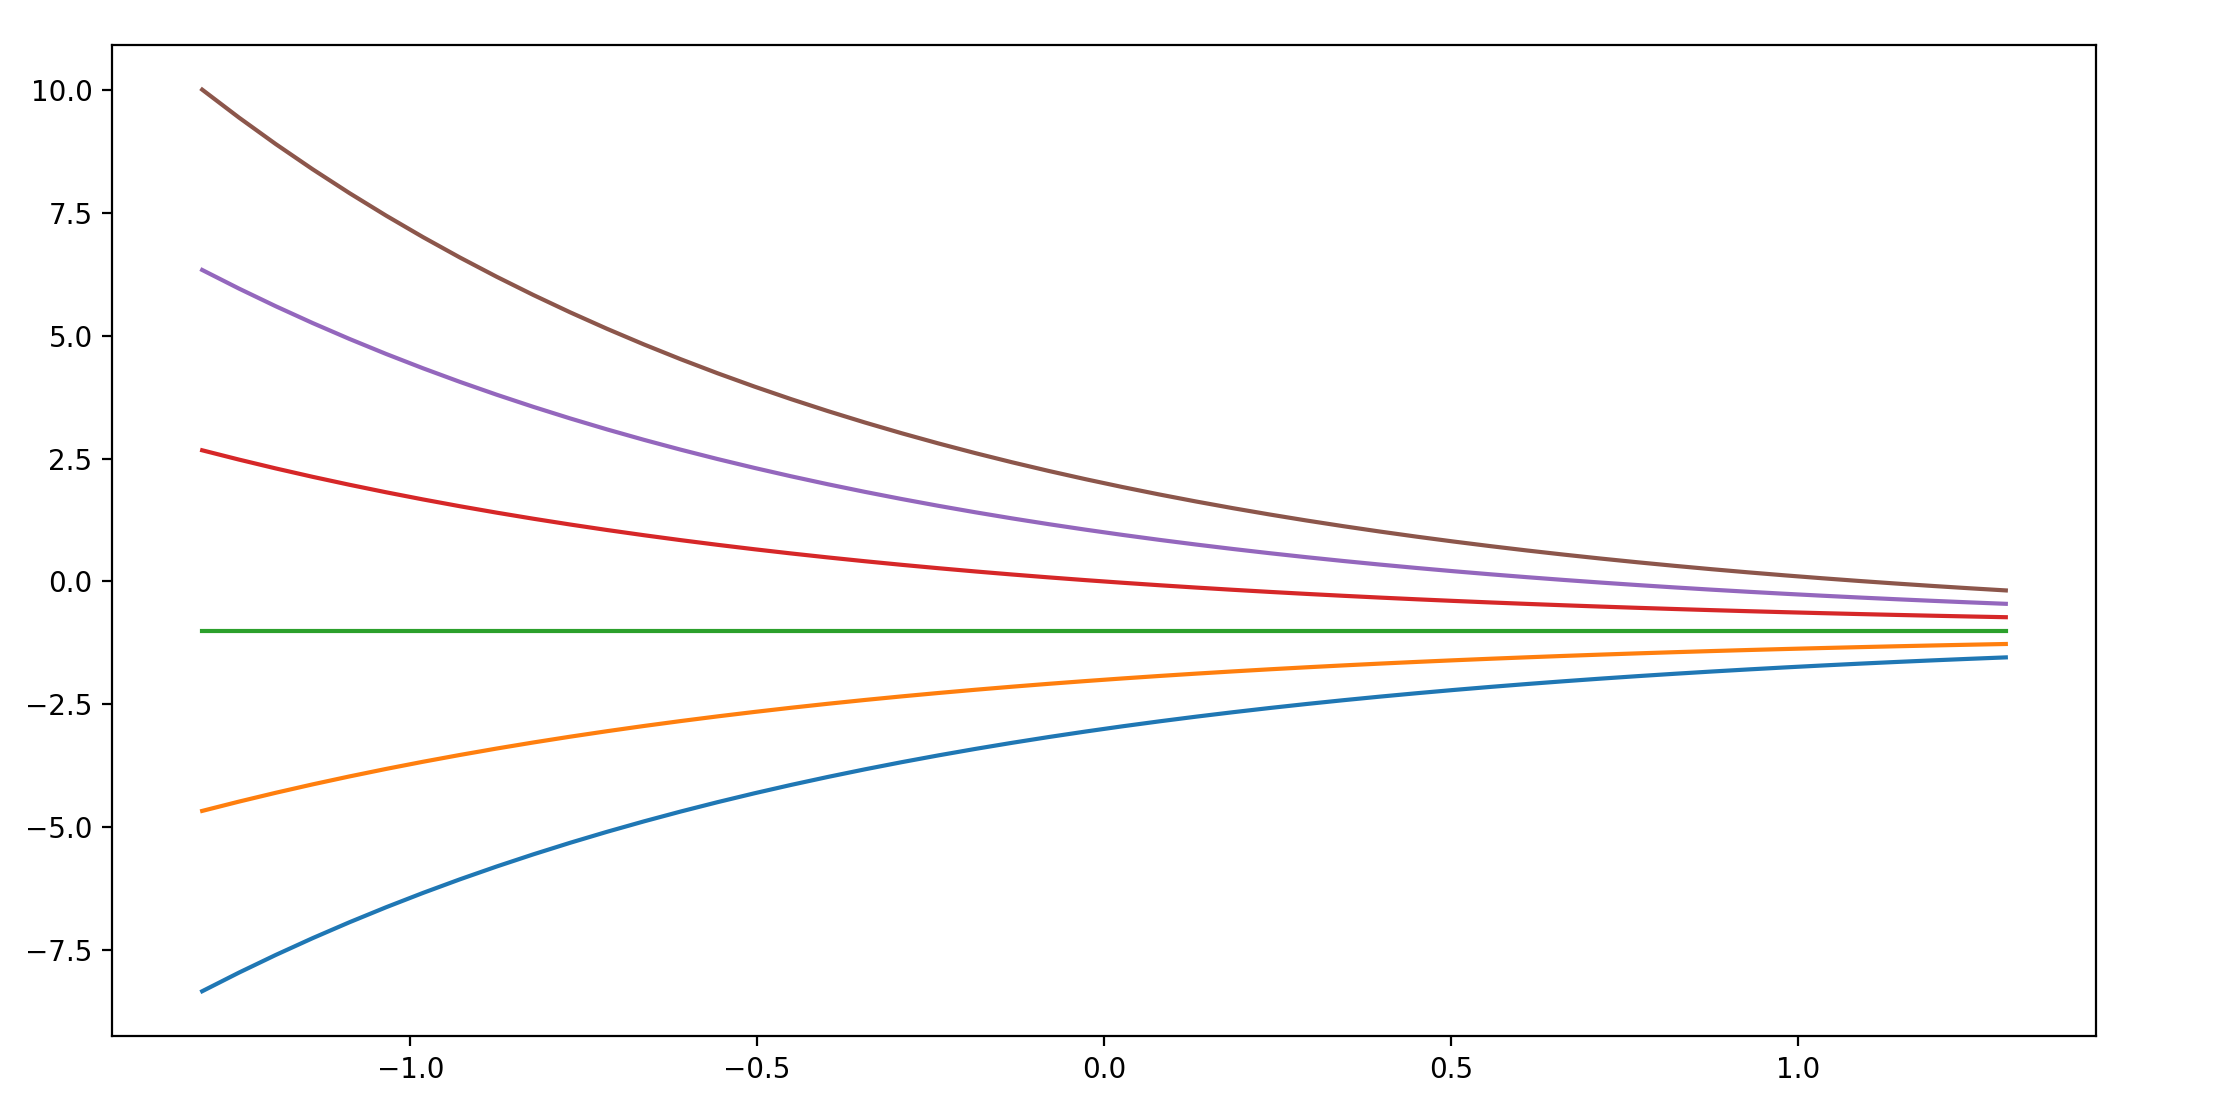
\includegraphics[scale=0.2]{des1}
\end{center}
\columnbreak
\begin{center}
$a=-1$ et $y(0) \in \lbrace -3,-2,-1,0,1,2 \rbrace$
\end{center}

\begin{center}
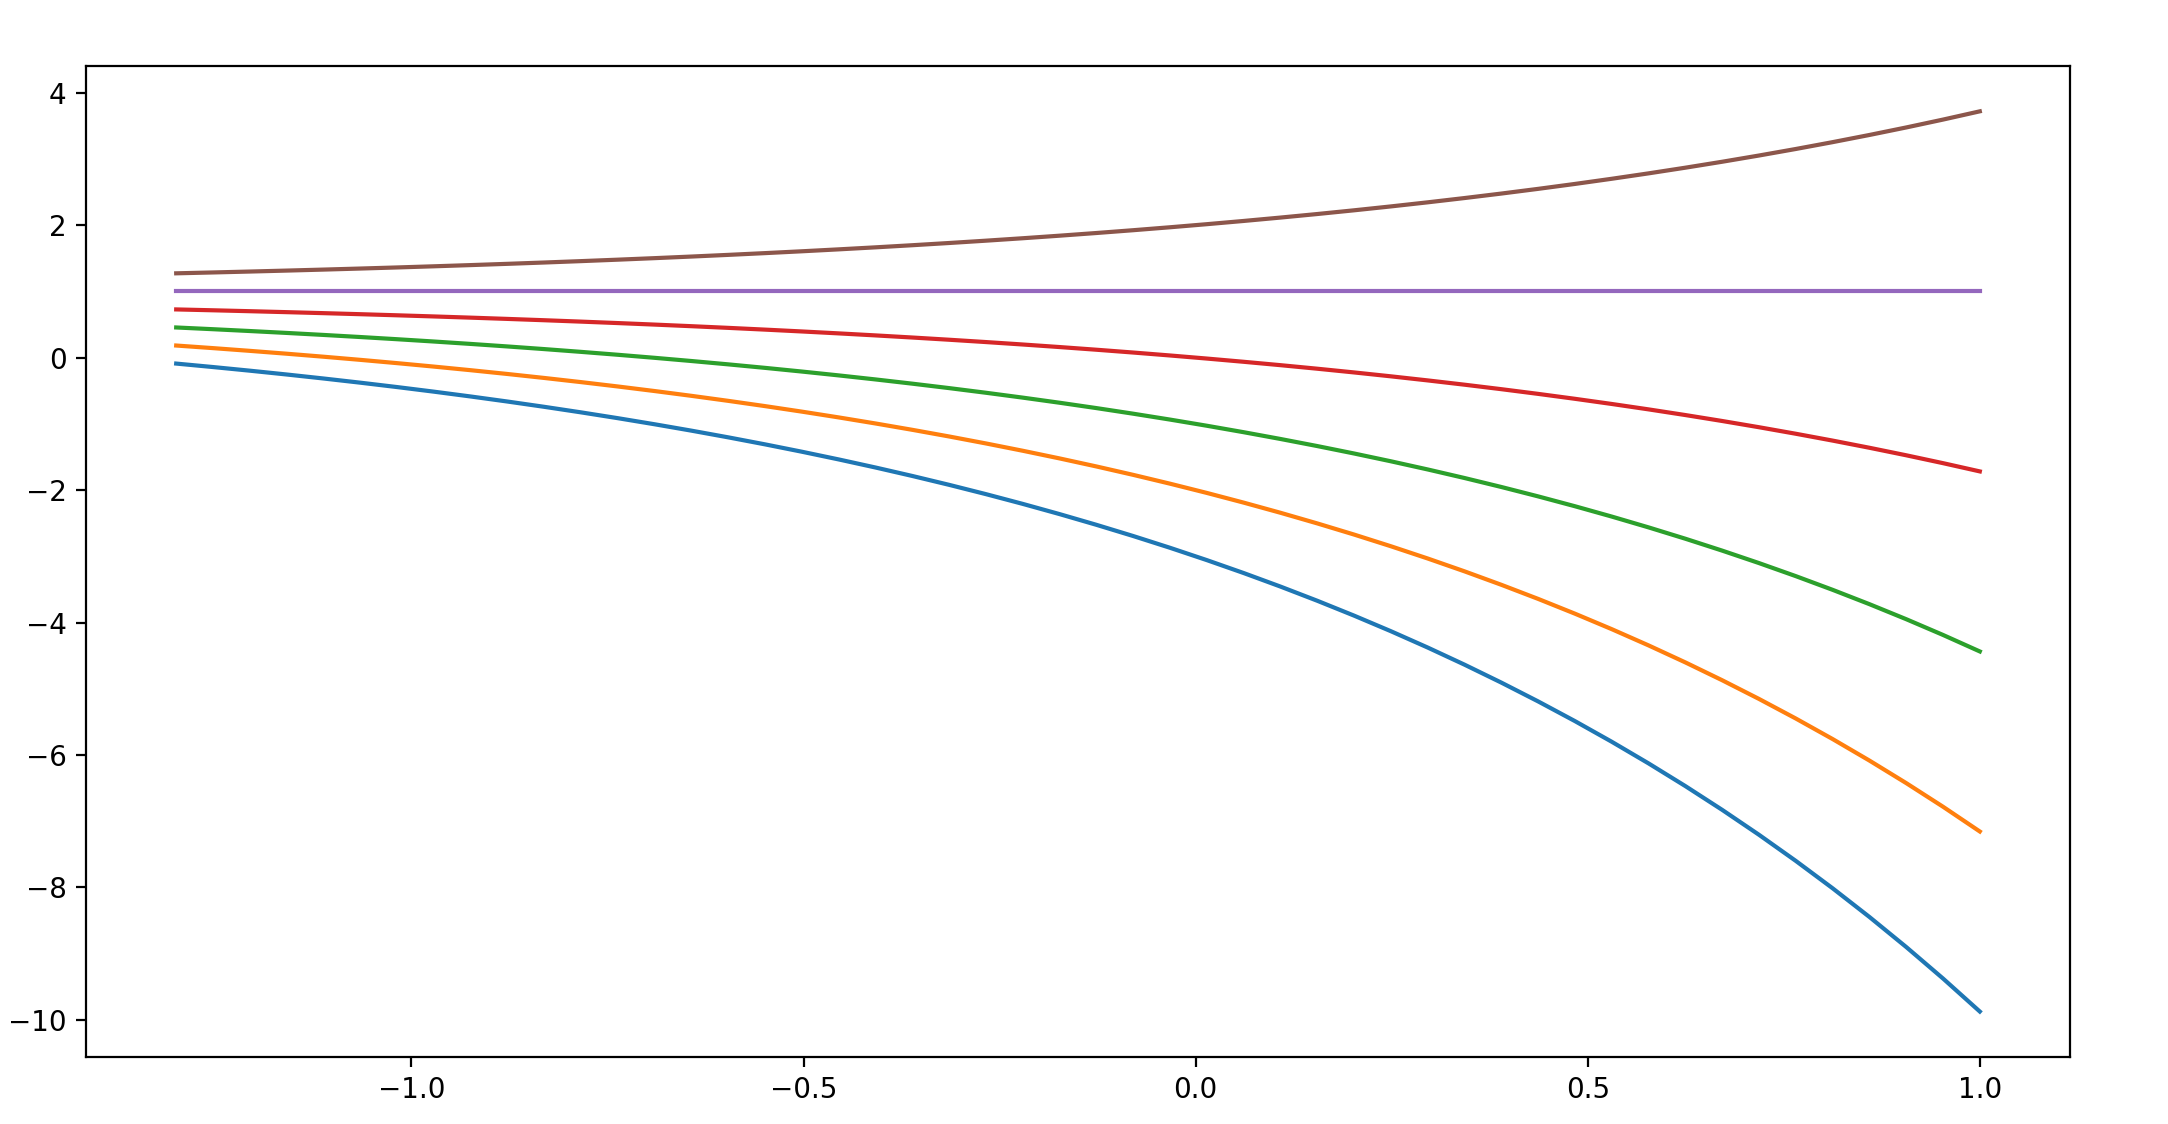
\includegraphics[scale=0.2]{des2}
\end{center}
\end{multicols}

\subsection{Résolution de l'équation homogène}
\noindent Considérons l'équation différentielle linéaire d'ordre $1$ homogène suivante : 
$$(\mathcal{E}_H) \quad   y'+a y= 0 $$
où $a : I \rightarrow \mathbb{K}$ est une fonction continue. 

\begin{prop} Soit $A$ une primitive de $a$ sur $I$ (qui existe car $a$ est continue sur $I$). Les solutions de $(\mathcal{E}_H)$ sont les fonctions :
$$ \begin{array}{cclcc}
y & : & I & \rightarrow & \mathbb{K} \\
 & & t & \mapsto & \lambda e^{-A(t)} \\
\end{array}$$
où $\lambda \in \mathbb{K}$.
\end{prop}

\begin{preuve}

\vspace{4cm}
\end{preuve}

\begin{rem} En notant $f_h=\exp \circ (-A)$, l'ensemble des solutions $\mathcal{S}_H$ de $(\mathcal{E}_H)$ est défini par :
$$ \mathcal{S}_H = \lbrace \lambda f_h \, \vert \, \lambda \in \mathbb{K} \rbrace = \textrm{Vect}_{\mathbb{K}}(f_h)$$
\end{rem}

\begin{ex} Résolvons l'équation différentielle suivante sur $]-1, + \infty[$ :
$$ y'+ \frac{y}{1+t}= 0 $$

\vspace{4cm}
\end{ex}

\subsection{Résolution de l'équation avec une solution particulière}
\noindent Considérons l'équation différentielle linéaire du premier ordre suivante : 
$$(\mathcal{E}) \quad  y'+a y= b $$
où $a : I \rightarrow \mathbb{K}$ et $b : I \rightarrow \mathbb{K}$ sont des fonctions continues.

\begin{prop} Soient $f_p$ une solution particulière de $(\mathcal{E})$ (qui existe d'après le théorème de Cauchy-Lipschitz linéaire) et $A$ une primitive de $a$ sur $I$. Les solutions de $(\mathcal{E})$ sont les fonctions :
$$ \begin{array}{cclcl}
y & : & I & \rightarrow & \mathbb{K} \\
 & & t & \mapsto &  f_p(t) +\lambda e^{-A(t)} \\
\end{array}$$
où $\lambda \in \mathbb{K}$.
\end{prop}

\begin{preuve}

\vspace{4cm}
\end{preuve}

\begin{rem} En notant $f_h=\exp \circ (-A)$ et $f_p$ une solution particulière de $E$, l'ensemble des solutions $\mathcal{S}$ de $(\mathcal{E})$ est défini par :
$$ \mathcal{S} = \lbrace f_p + \lambda f_h  \, \vert \, \lambda \in \mathbb{K} \rbrace$$
On utilise parfois la notation affine :
$$  \mathcal{S} = f_p + \textrm{Vect}_{\mathbb{K}}(f_h)$$
qui signifie que tout élément de $S$ s'écrit comme $f_p$ plus un élément de $\textrm{Vect}_{\mathbb{K}}(f_h)$.
\end{rem}

\medskip

\begin{ex} Résolvons l'équation différentielle suivante sur $]-1, + \infty[$ :
$$ y'+ \frac{y}{1+t}= \dfrac{1}{1+t} $$

\vspace{4cm}
\end{ex}

\subsection{Comment déterminer une solution particulière ?}

\medskip

\noindent \textbf{Méthode 1 : cas où $a$ est constante non nulle}

\begin{enumerate}
\item \textit{Technique d'annulation de la dérivée de Mme Boivin} : si $b$ est aussi constante, $t \mapsto \dfrac{b}{a}$ est une solution évidente.
\item Si $b$ est une fonction polynômiale de degré supérieur ou égal à $1$, on peut chercher comme solution particulière une fonction polynomiale même degré que $b$.
\end{enumerate}

\medskip

\begin{ex} Résolvons l'équation différentielle suivante :
$$ y'-y = t^2+2t-3$$

\vspace{5cm}
\end{ex}

\pagebreak

$\phantom{test}$

\vspace{2cm}

\begin{exa} Résoudre l'équation différentielle suivante : $y'-2y=5t+2$.
\end{exa}

\medskip

\noindent \textbf{Méthode 2 : variation de la constante}

\noindent Considérons l'équation différentielle linéaire du premier ordre suivante : 
$$(\mathcal{E}) \quad y'+a y= b $$
où $a : I \rightarrow \mathbb{K}$ et $b : I \rightarrow \mathbb{K}$ sont des fonctions continues.

\noindent Les solutions de l'équation homogène associée sont les fonctions définies sur $I$ de la forme $t \mapsto \lambda \exp \circ(-A)$. Il suffit alors de chercher une solution particulière sous la forme $t \mapsto \lambda(t) e^{-A(t)}$ où $\lambda : I \rightarrow \mathbb{K}$ est une fonction dérivable sur $I$.

\medskip

\begin{ex} Résoudre $y'+y= \ch(t)$.

\vspace{12cm}
\end{ex}

\begin{exa} Résoudre, sur $]0,\pi[$, l'équation différentielle $y' + \dfrac{\cos(t)}{\sin(t)}y=1$
\end{exa}

\medskip

\noindent \textbf{Méthode 3 : principe de superposition}

\noindent Soient $b_1 : I \rightarrow \mathbb{K}$ et $b_2 : I \rightarrow \mathbb{K}$ deux fonctions continues sur $I$ et $(\lambda_1, \lambda_2) \in \mathbb{K}^2$.

\noindent Si $y_1$ (resp. $y_2$) est une solution de $y'+ay=b_1$ (resp. $y'+ay=b_2$) alors $\lambda_1 y_1 + \lambda_2 y_2$ est une solution de $y'+ay=\lambda_1 b_1+ \lambda_2 b_2$.

\medskip

\pagebreak
\begin{ex} Résoudre, sur $\mathbb{R}$, l'équation $y'+y = \cos(t)$.

\vspace{10cm}
\end{ex}


\subsection{Problème de raccord}
\noindent Revenons à une équation différentielle du type :
$$ (\mathcal{E}) \, : \, \alpha y'+\beta y= \gamma$$
où $\alpha$, $\beta$ et $\gamma$ trois fonctions définies sur $I$. Si $\alpha$ s'annule sur $I$, on suit la méthode suivante :

\begin{enumerate}
\item On résout $(\mathcal{E})$ sur les plus grands (au sens de l'inclusion) intervalles $J \subset I$ où $a$ ne s'annule pas.
\item On raisonne ensuite par analyse-synthèse : 
\begin{itemize}
\item On suppose l'existence d'une solution $y$ de $(\mathcal{E})$ sur $I$. On connait son expression en tout point où $a$ ne s'annule pas.
\item Cette solution est continue et dérivable en tout point de $I$ : cela donne des conditions sur $y$.
\item La synthèse permet d'obtenir l'ensemble des solutions (si il y en a : il peut tout se passer !).
\end{itemize}
\end{enumerate}

\medskip

\begin{ex} Résolvons $ty'-y=t^2$ sur $\mathbb{R}$.
\vspace{10cm}
\end{ex}

\phantom{test}

\vspace{4cm}
\begin{exa} Résoudre sur $\mathbb{R}$ l'équation :
  \[
  (\e^{t} - 1)y' + \e^{t} y = 1
  \]
\end{exa}

\section{Systèmes différentiels linéaires d'ordre $1$}
\subsection{Une remarque}
\noindent Dans la suite, nous considérerons des fonctions définies sur un intervalle $I$ à valeurs dans $\mathcal{M}_{n,p}(\mathbb{R})$ de la forme :
$$ A : t \mapsto \begin{pmatrix}
a_{1,1}(t) & a_{1,2}(t) & \cdots & a_{1,p}(t)  \\
a_{2,1}(t) & a_{2,2}(t) & \cdots & a_{2,p}(t)  \\
\vdots & & \cdots & \vdots \\
a_{n,1}(t) & a_{n,2}(t) & \cdots & a_{n,p}(t)  \\
\end{pmatrix}$$
La fonction $A$ est continue sur $I$ si et seulement si toutes les fonctions coefficients $a_{i,j}$ le sont. La fonction $A$ est dérivable sur $I$ si et seulement si toutes ses fonctions coefficients le sont. On a dans ce cas pour tout $t \in I$,
$$ A'(t) = \begin{pmatrix}
a_{1,1}'(t) & a_{1,2}'(t) & \cdots & a_{1,p}'(t)  \\
a_{2,1}'(t) & a_{2,2}'(t) & \cdots & a_{2,p}'(t)  \\
\vdots & & \cdots & \vdots \\
a_{n,1}'(t) & a_{n,2}'(t) & \cdots & a_{n,p}'(t)  \\
\end{pmatrix}$$
On généralise pour définir $A$ de classe $\mathcal{C}^1$ sur $I$, $\mathcal{C}^2$ sur $I$...

\subsection{Définition}

\begin{defin}[Système différentiel linéaire d'ordre 1] Soient $A : I \rightarrow \mathcal{M}_n(\mathbb{K})$ et $B : I \rightarrow \mathcal{M}_{n,1}(\mathbb{K})$ deux applications continues. L'équation :
$$ (\mathcal{E}) \quad X'=A(t)X+B(t)$$
est appelée \textit{système différentiel linéaire d'ordre} $1$, d'inconnue $X$.

\noindent Une \textit{solution} de $(\mathcal{E})$ est une fonction $X : I \rightarrow \mathcal{M}_{n,1}(\mathbb{K})$ telle que pour tout $t \in I$,
$$ X'(t) = A(t) X(t) + B(t)$$
\end{defin}

\begin{rem}
On peut aussi définir une solution comme un couple $(X,J)$ où $X$ est solution du système différentiel uniquement sur un sous-intervalle $J \subset I$.
\end{rem}

\begin{defin} Reprenons les notations de la définition précédente.

\begin{itemize}
\item Le système $(\mathcal{E})$ est dit \textit{homogène} si $B$ est la fonction nulle de $I$ dans $\mathcal{M}_{n,1}(\mathbb{K})$.
\item Le système $(\mathcal{E})$ est dit \textit{à coefficients constants} si $A$ ne dépend pas de $t$.
\end{itemize}
\end{defin}

\begin{ex} Le système défini par :
$$ (\mathcal{E}) \quad \left\lbrace \begin{array}{lcl}
x_1'=x_1+x_2 + e^t \\
x_2'=x_1+2x_1 - e^{-t} \\
\end{array}\right.$$
peut se réécrire $X'=A(t)X+B(t)$ en posant :
$$ X(t) = \begin{pmatrix}
x_1(t) \\
x_2(t) \\
\end{pmatrix}, \; A(t) = \begin{pmatrix}
1 & 1 \\
1 & 2 \\
\end{pmatrix} \; \hbox{ et } \; B(t) = \begin{pmatrix}
e^t \\
-e^{-t} \\
\end{pmatrix}$$
Ce système est à coefficients constants.
\end{ex}

\subsection{Problème de Cauchy}
\begin{defin} On appelle \textit{problème de Cauchy} tout système de la forme :
$$ \left\lbrace \begin{array}{l}
X'=A(t)X+B(t) \\
X(t_0)=Y_0 \\
\end{array}\right.$$
où :
\begin{itemize}
\item $A$ et $B$ sont des fonctions définies sur $I$ à respectivement à valeurs dans $\mathcal{M}_n(\mathbb{K})$ et $\mathcal{M}_{n,1}(\mathbb{K})$.
\item $t_0$ est un élément de $I$ et $Y_0$ est un élément de $\mathcal{M}_{n,1}(\mathbb{K})$.
\end{itemize}
\end{defin}

\begin{thm}[Cauchy-Lipschitz linéaire] Si $A$ et $B$ sont des fonctions continues sur $I$ alors le problème de Cauchy précédent admet une unique solution.
\end{thm}

\subsection{Ensemble des solutions d'un système homogène}

\begin{prop} Considérons le système différentiel linéaire d'ordre $1$ homogène suivant :
$$ (\mathcal{E}) \quad X'=A(t)X$$
où $A : I \rightarrow \mathcal{M}_n(\mathbb{K})$ est une application continue. Notons $\mathcal{S}_H$ l'ensemble des solutions de $(\mathcal{E})$. Alors :

\begin{itemize}
\item $\mathcal{S}_H$ est un sous-espace vectoriel de $\mathcal{C}^1(I, \mathcal{M}_{n,1}(\mathbb{K}))$.
\item Pour tout $t_0 \in I$, l'application $E_{t_0}$ définie par :
$$ \begin{array}{cclll}
E_{t_0} & : & \mathcal{S}_H & \rightarrow & \mathcal{M}_{n,1}(\mathbb{K}) \\
& & X & \mapsto & X(t_0) \\
\end{array}$$
est un isomorphisme d'espaces vectoriels. 
\item $\mathcal{S}_H$ est de dimension $n$.
\end{itemize}
\end{prop}

\begin{preuve}

\vspace{8cm}
\end{preuve}

\begin{ex} Tout système de la forme :
$$ \left\lbrace \begin{array}{cclll}
x_1'= ax_1+bx_2 \\
x_2'= c x_1+dx_2 \\
\end{array}\right.$$
où $a$, $b$, $c$ et $d$ sont des fonctions continues de $I$ dans $\mathbb{K}$, a un ensemble solution qui est un plan vectoriel.
\end{ex}

\begin{rem} Si on connait une famille \textit{libre} de solutions de $E$, $(X_1, \ldots, X_n)$, alors cette famille est génératrice de $\mathcal{S}_H$ (argument de dimension) et ainsi :
$$ \mathcal{S}_H= \textrm{Vect}_{\mathbb{K}}(X_1, \ldots, X_n) = \lbrace \lambda_1 X_1 + \cdots + \lambda_n X_n \, \vert \, (\lambda_1, \ldots, \lambda_n) \in \mathbb{K}^n \rbrace$$
\end{rem}

\begin{exa} Résoudre le système différentiel suivant : 
$$ \left\lbrace \begin{array}{lclll}
x_1'= (2-t)x_1+(t-1) x_2 \\
x_2'= 2(1-t)x_1 +(2t-1)x_2 \\
\end{array}\right.$$
On pourra utiliser $(\exp,\exp)$ et $(f,2f)$ où $f : t \mapsto e^{t^2/2}$.
\end{exa}
\subsection{Ensemble des solutions du système avec une solution particulière} 
\begin{prop}\label{sol}
Considérons le système différentiel suivant : 
$$ (\mathcal{E}) \quad X'=A(t)X+B(t)$$
où $A : I \rightarrow \mathcal{M}_n(\mathbb{K})$ et $B : I : \rightarrow \mathcal{M}_{n,1}(\mathbb{K})$ sont des applications continues. Si $X_p$ est une solution particulière de $(\mathcal{E})$ (qui existe d'après le théorème de Cauchy-Lipschitz linéaire) alors les solutions de $(\mathcal{E})$ sont les applications de la forme :
$$ \begin{array}{llcll}
X &:&  I & \rightarrow & \mathcal{M}_{n,1}(\mathbb{K}) \\
& & t & \mapsto & X_p(t) + X_h(t) \\
\end{array}$$
où $X_h$ est une solution de l'équation homogène associée à $(\mathcal{E}$).
\end{prop}


\begin{preuve}
\vspace{4cm}
\end{preuve}

\begin{rem} L'ensemble des solutions $\mathcal{S}$ de $(\mathcal{E})$ est défini par :
$$ \mathcal{S} = \lbrace X_p + \lambda_1 Y_1 + \cdots + \lambda_n Y_n  \, \vert \, (\lambda_1, \ldots, \lambda_n) \in \mathbb{K}^n \rbrace$$
où $(Y_1, \ldots, Y_n)$ est une base de $\mathcal{S}_H$. En utilisant la notation affine, on a :
$$  \mathcal{S} =X_p + \textrm{Vect}_{\mathbb{K}}(Y_1, \ldots, Y_n)$$
qui signifie que tout élément de $S$ s'écrit comme $X_p$ plus un élément de $\mathcal{S}_H$.
\end{rem}

\section{Systèmes différentiels linéaires d'ordre $1$ à coefficients constants}
\noindent Dans cette section, on considère le système différentiel linéaire d'ordre $1$ suivant :
$$ (\mathcal{E}) \quad X'=AX+B(t)$$
où $A \in \mathcal{M}_n(\mathbb{K})$ et $B : I  \rightarrow \mathcal{M}_{n,1}(\mathbb{K})$.
On note $(\mathcal{E}_H)$ le système homogène associé.
\subsection{Premier cas : si $A$ est diagonalisable}
\noindent Dans ce cas, il existe une matrice $D \in \mathcal{M}_n(\mathbb{K})$ diagonale et une matrice $P \in \mathcal{M}_n(\mathbb{K})$ inversible telles que :
$$ A=PDP^{-1}$$
On a $D= \textrm{diag}(\lambda_1, \ldots, \lambda_n)$ où les $\lambda_i$ sont les valeurs propres de $A$ (éventuellement avec répétitions).

\medskip

\noindent \textbf{Cas homogène :} Notons $\mathcal{S}_H$ l'ensemble des solutions de $(\mathcal{E}_H)$. Soit $X : I \rightarrow \mathbb{K}$ une application dérivable. Alors :
\begin{align*}
X \in \mathcal{S}_H & \Longleftrightarrow  X'=AX \\
& \Longleftrightarrow X'=PDP^{-1} X\\
& \Longleftrightarrow P^{-1}X'=DP^{-1}X \\
& \Longleftrightarrow (P^{-1}X)'=D(P^{-1}X) \\
& \Longleftrightarrow \left\lbrace \begin{array}{l}
Y=P^{-1}X \\
Y'=DY \\
\end{array}\right. \\
& \Longleftrightarrow \left\lbrace \begin{array}{l}
Y=P^{-1}X \\
\forall i \in \Interv{1}{n}, \; \forall t \in  \mathbb{R},  \; y_i'(t)=\lambda_i y_i(t)  \\
\end{array}\right. \qquad \qquad \hbox{ où } Y= ~^t(y_1, \ldots, y_n) \\
& \Longleftrightarrow \left\lbrace \begin{array}{l}
X=PY \\
\forall i \in \Interv{1}{n}, \; \exists c_i \in  \mathbb{R} \, \vert \, \forall t \in \mathbb{R}, \; y_i(t)=c_i e^{\lambda_i t}  \\
\end{array}\right.
\end{align*}
Il suffit alors de calculer $PY$ pour obtenir l'ensemble des solutions $\mathcal{S}_H$.

\begin{rem} Il n'est pas nécessaire de connaitre $P^{-1}$ dans ce cas.
\end{rem}

\begin{ex} Résolvons le système différentiel linéaire d'ordre $1$ à coefficients constants suivant : 
$$ \left\lbrace \begin{array}{lll}
    x' & = 4x - 2y \\
    y' & = x + y \\
    \end{array}\right.$$
    
    \vspace{12cm}
\end{ex}

\begin{exa} Résoudre le système différentiel suivant :
$$ \left\lbrace \begin{array}{lll}
     x'&=y+z \\
    y' & =x \\
     z'&=x+y+z \\
    \end{array}\right.$$

\end{exa}
\medskip

\noindent \textbf{Cas non homogène :} 
\begin{itemize}
\item Si on connait une solution particulière, on connait alors l'ensemble des solutions d'après la proposition (\ref{sol}) (il suffit de résoudre le système homogène).
\item Sinon, on utilise la même méthode que précédemment mais en gardant le second membre $B$ :
\begin{align*}
X \in \mathcal{S} & \Longleftrightarrow  X'=AX+B \\
& \Longleftrightarrow X'=PDP^{-1} X+B\\
& \Longleftrightarrow P^{-1}X'=DP^{-1}X + P^{-1}B\\
& \Longleftrightarrow (P^{-1}X)'=D(P^{-1}X) + P^{-1}B \\
& \Longleftrightarrow \left\lbrace \begin{array}{l}
Y=P^{-1}X \hbox{ et }  C=P^{-1}B\\
Y'=DY+C \\
\end{array}\right. \\
& \Longleftrightarrow \left\lbrace \begin{array}{l}
Y=P^{-1}X \hbox{ et }  C=P^{-1}B\\
\forall i \in \Interv{1}{n}, \; \forall t \in  \mathbb{R}, \, y_i'(t)=\lambda_i y_i(t) + c_i(t)  \\
\end{array}\right. \qquad \qquad \hbox{ où } Y= ~^t(y_1, \ldots, y_n) \hbox{ et } C= ~^t(c_1, \ldots, c_n)
\end{align*}
Chacune des équations différentielles est une équation différentielle linéaire du premier ordre dont on sait trouver les solutions (en utilisant par exemple la méthode de la variation de la constante).
\end{itemize}

\begin{rem} Dans le cas précédent, il devient nécessaire de déterminer expliciter $P^{-1}$.
\end{rem}
\medskip

\noindent \textbf{Cas où la matrice est diagonalisable dans $\mathbb{C}$} 

\noindent Dans ce cas, on diagonalise dans $\mathbb{C}$ et si l'on s'intéresse aux solutions à valeurs réelles, on cherche des conditions sur les constantes pour que les solutions vérifient cela.

\subsection{Deuxième cas : si $A$ est trigonalisable}

\noindent Dans ce cas, on adapte la méthode utilisée dans le cas où la matrice est diagonalisable. La détermination de $y_1$, $\ldots$, $y_n$ devient plus pénible : on trouve facilement $y_n$ (équation différentielle linéaire homogène), puis $y_{n-1}$ en utilisant l'expression de $y_n$ et on continue de proche en proche. 

\medskip

\begin{ex} Résolvons le système différentiel linéaire d'ordre $1$ à coefficients constants suivant : 
$$ \left\lbrace \begin{array}{lll}
    x' & = 3x + 2y \\
    y' & = -2x - y \\
    \end{array}\right.$$
\end{ex}

\vspace{10cm}

\newpage

$\phantom{test}$

\vspace{6cm}
\section{Équations différentielles linéaires scalaires d'ordre $2$}

\noindent On s'intéresse dans cette section à une équation différentielle linéaire d'ordre deux de la forme :
$$ (\mathcal{E}) \quad x''+a(t)x'+b(t)=c(t)$$
où $a$, $b$ et $c$ sont trois fonctions continues de $I$ dans $\mathbb{K}$ et $x : I \rightarrow \mathbb{K}$ est l'inconnue (fonction $2$ fois dérivable sur $I$).

\medskip

\noindent Remarquons qu'une solution de $(\mathcal{E})$ est alors nécessairement de classe $\mathcal{C}^2$ sur $I$.


\subsection{Système différentiel associé}
\noindent Soit $x : I \rightarrow \mathbb{K}$ dérivable. Posons $X : I \rightarrow \begin{pmatrix}
x(t) \\
x'(t) \\
\end{pmatrix} \cdot$

\begin{itemize}
\item Si $x$ est solution de $(\mathcal{E})$ sur $I$ alors $X$ est dérivable sur $I$ et pour tout $t \in I$,
$$ X'(t) = \phantom{\begin{pmatrix}
x'(t) \\
x''(t) \\
\end{pmatrix} = \begin{pmatrix}
x'(t) \\
-a(t)x'(t)-b(t)x(t)+c(t) \\
\end{pmatrix} = \begin{pmatrix}
0 & 1 \\
-b(t) & - a(t) \\
\end{pmatrix} \begin{pmatrix}
x(t) \\
x'(t) \\
\end{pmatrix} + \begin{pmatrix}
0 \\
c(t)
\end{pmatrix}}$$
En posant pour tout $t \in I$,
$$ A(t) = \phantom{\begin{pmatrix}
0 & 1 \\
-b(t) & -a(t) \\
\end{pmatrix}} \; \hbox{ et } B(t) = \phantom{\begin{pmatrix}
0 \\
c(t)
\end{pmatrix}}$$
Alors $X$ est solution de $X'=A(t)X(t)+B(t)$ sur $I$.
\item Réciproquement si $X = \begin{pmatrix}
x \\
y \\
\end{pmatrix}$ est une solution de $X'=A(t)X(t)+B(t)$ sur $I$ alors pour tout $t \in I$,
$$\begin{pmatrix}
x'(t) \\
y'(t) \\
\end{pmatrix} =  \begin{pmatrix}
0 & 1 \\
-b(t) & - a(t) \\
\end{pmatrix} \begin{pmatrix}
x(t) \\
y(t) \\
\end{pmatrix} + \begin{pmatrix}
0 \\
c(t)
\end{pmatrix} = \begin{pmatrix}
y(t) \\
-a(t) y(t)-b(t)x(t)+c(t)
\end{pmatrix}$$
La première coordonnée précise que $y=x'$ donc $x$ est deux fois dérivable sur $I$ et $x''=y'$ et la deuxième coordonnée implique donc que pour tout $t \in I$,
$$ x''(t)= -a(t)x'(t)-b(t)x(t)+c(t)$$
et ainsi $x$ est solution de $(E)$ sur $I$.
\end{itemize}

\medskip

\noindent Le résultat prouvé est donc le suivant :

\begin{prop} Gardons les notations précédentes. Les solutions sur $I$ du système différentiel :
$$ X'= A(t)X+B(t) $$
sont les fonctions de la forme :
$$ \begin{pmatrix}
x \\
x' \\
\end{pmatrix}$$
où $x$ est solution de $(\mathcal{E})$. En particulier, les solutions de $(E)$ sont les premières fonctions coordonées des solutions de $X'=A(t)X+B(t)$.
\end{prop}

\begin{retenir} Pour résoudre une équation différentielle linéaire d'ordre deux, on peut se ramener à un système d'équation différentiel linéaire d'ordre $1$ (que l'on a étudié dans les sections précédentes).
\end{retenir}

\begin{ex} Donnons le système différentiel associé à l'équation suivante :
$$ x''+tx'+t^2x=t^3$$

\vspace{4cm}
\end{ex}

\begin{rem} On peut procéder de la même manière pour associer une équation différentielle linéaire d'ordre $n$ à un système différentiel de taille $n$ : voir TD.
\end{rem}

\medskip

\noindent Le théorème de Cauchy-Lipschitz linéaire connu dans dans le cas des systèmes différentiels s'adapte donc aux équations du même type que $(\mathcal{E})$.

\begin{thm} Soient $a$, $b$ et $c$ trois fonctions continues sur $I$ à valeurs dans $\mathbb{K}$.

\begin{itemize}
\item Pour tout $t_0 \in I$ et tout $(x_0,x_1) \in \mathbb{K}^2$, le problème de Cauchy :
$$ \left\lbrace \begin{array}{l}
(\mathcal{E}) \quad \forall t \in I, \; x''(t)+a(t)x'(t)+b(t)x(t) = c(t)  \\
x(t_0)=x_0 \\
x'(t_0) = x_1 \\
\end{array}\right.$$
possède une unique solution.
\item L'ensemble des solutions de l'équation homogène associé à $(\mathcal{E})$ est un plan vectoriel de $\mathcal{C}^2(I, \mathbb{K})$.
\item Les solutions de $(\mathcal{E})$ sont de la forme $f_p + f_h$ où $f_p$ est une solution particulière de $(\mathcal{E})$ et $f_h$ est une solution de l'équation homogène associée à $(\mathcal{E})$.
\end{itemize}
\end{thm}

\begin{rem} Il n'existe pas de méthode général pour résoudre ce type d'équation. On verra quelques cas particuliers en TD.
\end{rem}

\subsection{Cas particulier : équation à coefficients constants}

\noindent On s'intéresse dans cette sous-section à une équation différentielle linéaire d'ordre deux de la forme :
$$ (\mathcal{E}) \quad x''+ax'+b=c(t)$$
où $a$ et $b$ sont deux réels et $c$ une fonction continue de $I$ dans $\mathbb{K}$.

\medskip

\noindent Notons $(\mathcal{E}_H)$ l'équation homogène associée à $(\mathcal{E})$ et $\mathcal{S}_H$ l'ensemble des solutions associé.

\medskip

\noindent Le cours de première année permet de déterminer $\mathcal{S}_H$ : il suffit pour cela de s'intéresser à l'équation caractéristique, notée $(EC)$, associée à $(\mathcal{E}_H)$ :
$$ z^2+az+b=0 \hbox{ où } z \in \mathbb{K}$$

\begin{prop} 
\begin{itemize}
\item Si $(EC)$ admet deux solutions distinctes $r_1$ et $r_2$ dans $\mathbb{K}$ alors $t \mapsto e^{r_1 t}$ et $t \mapsto e^{r_2 t}$ forment une base de $\mathcal{S}_H$. Ainsi, $x : I \rightarrow \mathbb{K}$ est solution de $(\mathcal{E}_H)$  si et seulement si il existe $(\lambda, \mu) \in \mathbb{K}^2$ tel que pour tout $t \in I$,
$$ x(t) = \lambda e^{r_1 t} + \lambda e^{r_2 t} $$
\item Si $(EC)$ admet une racine double $r_0$ dans $\mathbb{K}$ alors $t \mapsto e^{r_0 t}$ et $t \mapsto t e^{r_0 t}$ forment une base de $\mathcal{S}_H$. Ainsi, $x : I \rightarrow \mathbb{K}$ est solution de $(\mathcal{E}_H)$ si et seulement si il existe $(\lambda, \mu) \in \mathbb{K}^2$ tel que pour tout $t \in I$,
$$ x(t) =  (\lambda + \mu t)e^{r_0 t}  $$
\item Cas où $\mathbb{K}= \mathbb{R}$ : Si $(EC)$ admet deux racines complexes conjuguées $\alpha \pm i \beta$ alors $t \mapsto e^{\alpha t} \cos(\beta t)$ et $t \mapsto e^{\alpha t} \sin(\beta t)$ forment une base de $\mathcal{S}_H$. Ainsi, $x : I \rightarrow \mathbb{R}$ est solution de $(\mathcal{E}_H)$ si et seulement si il existe $(\lambda, \mu) \in \mathbb{R}^2$ tel que pour tout $t \in I$,
$$ x(t) = (\lambda \cos(\beta t) + \mu \sin( \beta t)) e^{\alpha t} $$
\end{itemize}
\end{prop}

\begin{rem} Le système différentiel associé à $(\mathcal{E}_H)$ est $X'=AX$ où :
$$ A = \begin{pmatrix}
0 & 1 \\
-b & -a
\end{pmatrix}$$
Le polynôme caractéristique de cette matrice est $X^2+aX+b$ ce qui justifie la notion d'équation caractéristique. En étudiant la diagonalisabilité ou la trigonalisabilité de $A$, on peut retrouver le résultat précédent à l'aide des méthodes de la section précédente.
\end{rem}

\begin{ex} Résolvons sur $\mathbb{R}$ l'équation différentielle $y''+2y'+2=0$.

\vspace{4cm}
\end{ex}

\subsection{Obtention d'une solution particulière pour les équations à coefficients constants}
\noindent On s'intéresse dans cette section à une équation différentielle linéaire d'ordre deux de la forme :
$$ (\mathcal{E}) \quad x''+ax'+b=c(t)$$
où $a$ et $b$ sont deux réels et $c$ une fonction continue de $I$ dans $\mathbb{K}$.

\medskip

\noindent Voici quelques méthodes pour déterminer une solution particulière : 

\begin{itemize}
\item Si $c$ est de la forme $t \mapsto C e^{\alpha t}$ où $(C, \alpha) \in \mathbb{K}^2$ alors on peut déterminer une solution particulière de $(E)$ sous la forme :
\begin{enumerate}
\item $t \mapsto A e^{\alpha t}$ si $\alpha$ n'est pas solution de $(EC)$.
\item $t \mapsto At e^{\alpha t}$ si $\alpha$ est une solution \og simple \fg de $(EC)$.
\item $t \mapsto At^2 e^{\alpha t}$ si $\alpha$ est solution \og double \fg $(EC)$.
\end{enumerate}
\item Si $\mathbb{K}= \mathbb{R}$ et si $c$ est de la forme $t \mapsto C \cos(\alpha t)$ ou $t \mapsto C \sin(\alpha t)$ avec $(C, \alpha) \in \mathbb{K}^2$ alors on détermine une solution particulière de l'équation suivante :
$$ x''+ax+b= e^{i \alpha t}$$
en se ramenant au cas précédent puis on considère la partie réelle ou imaginaire de cette solution particulière.
\item Le principe de superposition s'adapte aussi dans ce cadre.
\end{itemize}

\begin{ex} Résoudre $y'' + 3y' + 2y = \ch(t)$.

\vspace{10cm}
\end{ex}

\newpage

$\phantom{test}$

\vspace{10cm}

\begin{ex} Résoudre $y''+2y'+y= \cos(t)$.

\vspace{10cm}
\end{ex}

\begin{exa} Déterminer les solutions réelles de l'équation :
  \[
   y'' - 3y' + 2y = \sin(2x)
  \]
\end{exa} 
\subsection{Que faire si le second membre n'est pas \og simple \fg ? (pleurer n'est pas une solution)}
\noindent Dans ce cas, d'après le programme, une indication doit être donnée.

\medskip

\begin{ex} Résoudre sur $\mathbb{R}$ l'équation différentielle suivante :
$$ x''+6x'+9x= \dfrac{e^{-3t}}{1+t^2}$$
On cherchera une solution sous la forme $t \mapsto b(t)e^{-3t}$ où $b$ est une fonction dérivable sur $\mathbb{R}$.

\vspace{11cm}
\end{ex}

%\begin{rem} On verra dans le TD quelques méthodes de résolution dans des cas particuliers.
%\end{rem}

\subsection{Problème de raccord}
\noindent Si l'équation donnée est de la forme :
$$ \alpha(t) y''+ \beta(t) y'+ \gamma(t) = \delta(t)$$
et que la fonction $\alpha$ s'annule sur $I$ : on adapte la méthode donnée dans le cas de l'ordre $1$ : la nuance est d'utiliser (probablement) la dérivabilité d'ordre deux de (ou des) solution(s) éventuelle(s) (dans la phase d'analyse).
\section{Utilisation des séries entières}
\noindent Supposons que l'on souhaite résoudre une équation différentielle linéaire du premier ordre ou du second ordre dont les coefficients sont des fonctions polynômiales (ou développables en séries entières). On peut dans ce cas supposer l'existence d'une solution de cette équation développable en série entière (raisonnement par analyse-synthèse) : on injecte celle-ci dans l'équation et cela donne des conditions sur les coefficients. La synthèse permet effectivement de conclure sur l'existence d'une solution (et le théorème de Cauchy-Lipschitz linéaire peut même préciser l'unicité si nous disposons de condition(s) initiale(s)).

\medskip

%Bibmath
\begin{ex} Considérons le problème de Cauchy suivant :
$$ y''+xy'+y=1 $$
avec $y(0)=y'(0)=0$. Ce problème de Cauchy a une unique solution d'après le théorème de Cauchy-Lipschitz linéaire. Déterminons cette unique solution.

\vspace{10cm}
\end{ex}

\newpage

$\phantom{test}$

\vspace{7cm}
\begin{exa}
Soit $f$ définie sur $]-1,1[$ par :
$$ f(x) = \dfrac{\arcsin(x)}{\sqrt{1-x^2}}$$
\begin{enumerate}
\item Justifier à l'aide d'un théorème que $f$ est développable en série entière sur $]-1,1[$.
\item Montrer que $f$ solution de :
$$ (1-x^2)y'-xy=1$$
\item Déterminer le développement en série entière de $f$ sur $]-1,1[$.
\end{enumerate}
\end{exa}

\end{document}